\documentclass{article}
\usepackage{listings}
\usepackage{amsmath}
\usepackage{graphicx}
\usepackage{float}
\usepackage{subcaption}
\usepackage[linewidth=1pt]{mdframed}
\usepackage[colorlinks]{hyperref}

\usepackage{algorithm}
\usepackage{algpseudocode}

\hypersetup{citecolor=DeepPink4}
\hypersetup{linkcolor=DarkRed}
\hypersetup{urlcolor=Blue}

\usepackage{cleveref}

\setlength{\parindent}{1em}
\setlength{\parskip}{1em}
\renewcommand{\baselinestretch}{1.0}

\begin{document}

\begin{titlepage}
	\centering
	{\scshape\LARGE Assignment 2\par}
	\vspace{1cm}
	{\scshape\Large Algorithms \& Complexity (CIS 522-01)\par}
	\vspace{1.5cm}
	{\Large\itshape Javier Arechalde\par}
	\vfill
	{\large \today\par}
\end{titlepage}

\section*{Stress Testing}

\subsection*{Model description}

In this problem, we are doing some stress-testing on various models of glass jars, to determine the highest distance they can be dropped without breaking. 

We have a ladder with $n$ rungs, and we want to find the \textit{highest safe rung}, that is the distance that we described in the last paragraph. We also have $k$ jars, and this number of available jars, will be limited depending on the "budget" for the test.

\subsection*{a.}

In this case our budget is limited to $k = 2$ and we want to find a solution $f(n)$ that grows slower than linearly. The breaking distance for the first jar $k_1$ is $bd$ and the breaking distance for the second jar $k_2$ is $bd$ too, as they are models of the same jar.

The current rung we are dropping our jars from is $r$, and the highest safe run will be assigned to $sr$.

\subsection*{Overall idea}

In case we are given 2 jars, $k = 2$, we will use one algorithm with a different approach, because if we use linear search, our solution will grow linearly, but if we use binary search, we will exceed the number of available jars we have for this problem.

In our implementation, we will try a different approach, so we make the best use of the two jars that we have available, while keeping our solution growing slower than linearly. We will divide the set of $n$ rungs into $m$ parts, each one of these parts containing $n/m$ parts.

First we will use the first jar iterating over the $m$ parts until the jar breaks, by steps of size $n/m$. Once the first jar breaks, we will then start from the previous rung (distanced $n/m$ from the rung on which the jar broke) with the next jar, increasing the rungs by $1$, then the maximum safe rung will be the previous rung on which the jar broke.
 
\subsection*{Pseudocode}

\begin{algorithm}[H]
\caption{My implementation}
\begin{algorithmic}[1]
\State At the beginning $r = 0$ and $k_1,k_2$ are not broken
\State We have $n$ rungs, and we chose to divide our rungs into $m = 4$
\While{$k_1$ not broken}
 \State Start increasing distance
 \State Saving last ring $r_0 = r$
 \State $r = r + n/m$
 \If{$r>bd$}
  \State $k_1$ breaks at rung r
 \EndIf
\EndWhile
\State We start our next iterations from r = r0
\While{$k_2$ not broken}
 \State r = r + 1
 \If{$r>bd$}
  \State We return $sr = r-1$, safest rung distance for the jars not to break
 \EndIf 
\EndWhile
\end{algorithmic}
\end{algorithm}

\subsection*{Example}

In this section, we will show our implementation, and we will run it over a sample set.

\lstinputlisting[language=Python]{Problem1a.py}

In the image shown below, you can see the results of running this algorithm over the sample set.

\begin{figure}[H]
\begin{center}
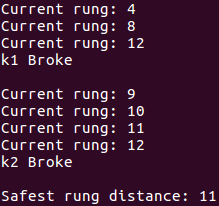
\includegraphics[scale=.8]{problem1a}
\end{center}
\caption{Results of running algorithm}
\end{figure}

\subsection*{Time complexity analysis}

As we stated before, in our solution, we will divide the ladder into $m$ divisions. This way, our algorithm will take $(m+n/m)$ steps at most, so then the time complexity of our implementation will be $O(m+n/m)$. This can be explained because in the worst case scenario, we will need to go over all the $m$ divisions to find the rung on which the first jar breaks, and then go to the start of the previous division before it broke, then iterate towards next division, on steps of $1$, which is $n/m$ steps away, at most, from the next division.

\subsection*{b.}

In this case, out budget is limited to $k$ jars, where $k>2$. We want to find the highest safe rung using at most $k$ jars. For each jar $k_i$ the number of times we drop whis jar should be less than the number of times we dropped the previous jar $k_{i-1}$ so $\lim_{n\to\infty} f_k(n)/f_{k-1}(n) = 0$.

The current rung we are dropping our jars from is $r$, and the highest safe run will be assigned to $sr$.

\subsection*{Overall idea}

In case we are given 2 jars, $k = 2$, we will use one algorithm with a different approach, because if we use linear search, our solution will grow linearly, but if we use binary search, we will exceed the number of available jars we have for this problem.

So in our solution, we will divide the ladder into $m$ divisions. This way, our algorithm will take $(m+n/m)$ steps at most. This can be explained because in the worst case scenario, we will need to go over all the $m$ divisions to find the highest safe rung, and then go to the start of the previous division before it broke, and go to the next division, which is $n/m$ steps away from the previous division.

\subsection*{Pseudocode}

\subsection*{Example}

\subsection*{Time complexity analysis}

\section*{Butterfly Studies}

\subsection*{Model description}

In this problem, we have $n$ butterflies, we want to separate then in two groups, let's call them $A$ and $B$. It doesn't matter in which group we classify each one of the butterflies, because we only want to separate them in two groups, we don't need to put them in the correct group.

To complete this task, we are given a $m$ comparisons that dictaminate if the pair of specimens $i,j$ belong to the same group, or they are in two separate groups. This number of $m$ comparisons, is smaller than the possible number of pairs in the set of specimens, which is $n(n-1)/2$, because some pairs are ambiguous, which means that we are not sure if the pair belongs to the same group or not.

We want to determine if this set of $m$ comparisons is consistant, and thus, we are separating the butterflies coherently.

\subsection*{Overall idea}

We will have a dictionary containing the $n$ different specimens that we want to separate. This way, we can check in only O(1), the group each specimen its assigned.

We will have a set of $m$ tuples that dictaminates if both specimens are in 'S' (Same group) or 'D' (different group). We also assume that this set of tuples comes in order, starting first with the pairs that contain specimen 1, then the pairs that contain specimen 2, etc.

We will start going tuple by tuple, if none of them have a group assigned, we will assign them to the same group, or to a different group, depending the notation on that tuple. If only one member of the tuple has a group assigned, we will assign the other tuple to the same group or the different one, according to the notation on that tuple. In the end, if both tuples have a group already assigned, we will proceed to check if this new notation is consistent or not. In the case it's not consistent, the whole classification is unconsistent, and we stop our algorihtm.

\subsection*{Pseudocode}

\begin{algorithm}[H]
\caption{My Implementation}
\begin{algorithmic}[1]
\While{The pairs are consistent, for every tuple in $m$}
 \State Take one tuple $m_i \in m$
 \If{None of the tuple members have a group assigned}
  \If{Tuple in the same group}
   \State Assign group $A$ to $m_i[0]$
   \State Assign group $A$ to $m_i[1]$
  \ElsIf{Tuple in different group}
   \State Assign group $A$ to $m_i[0]$.
   \State Assign group $B$ to $m_i[1]$.
  \EndIf
 \EndIf
 \If{One of the members in the tuple has a group assigned}
  \If{Tuple in the same group}
   \State Assign $Group(m_i[0])$ to $m_i[1]$
  \ElsIf{Tuple in different group}
   \State Assign opposite $Group(m_i[0])$ to $m_i[1]$
  \EndIf
 \EndIf
 \If{Both members on the tuple have a group assigned already}
  \If{Tuple in the same group}
   \If{They have different groups assigned}
    \State Inconsistency!
   \Else
    \State continue
   \EndIf
  \ElsIf{Tuple in different group}
   \If{They have same groups assigned}
    \State Inconsistency!
   \Else
    \State continue
   \EndIf
  \EndIf
 \EndIf
\EndWhile
\end{algorithmic}
\end{algorithm}

\subsection*{Example}

To prove that our algorithm works, we implemented it in Python, and we ran it over a sample dataset.

\lstinputlisting[language=Python]{problem2.py}


\subsection*{Time complexity analysis}

\end{document}
